\section{Trigger topology}

\subsection{Three level online trigger}

\begin{frame}{DAQ and trigger system}{Three levels to filter data}
	FPGA based L0 and software based L1 and L2 triggers:

	\begin{center} 
	\newcounter{counter}
	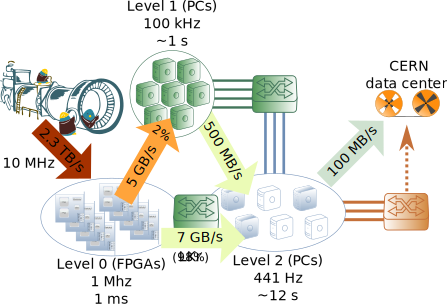
\includegraphics[width=0.9\textwidth]{data-mitigation.pdf}
	\end{center}
\end{frame}

\begin{frame}{First topology proposal}{}
	Original concept:
	\begin{center} 
		\includegraphics[width=0.7\textwidth]{double-star-en}
	\end{center}
\end{frame}

%\begin{frame}{Inhomogeneous L1: drawbacks}{}
%	\begin{block}{1 to 4 PCs \textbf{per detector}}		
%		\begin{itemize}
%		  \item	Inefficient scalability (spares?!)
%		\end{itemize}
%		\vspace{-0.4cm}
%		\begin{ergo}
%			All detectors should share the same computing power!
%		\end{ergo}
%	\end{block}
%	\begin{block}{One L1 program per detector}
%		\begin{itemize}
%		  \item	Difficult to maintain
%		\end{itemize}
%		\vspace{-0.4cm}
%		\begin{ergo}
%			All detectors should use the same protocols/framework!
%		\end{ergo}
%	\end{block}
	
%	\begin{exampleblock}{Solution: Install a homogeneous L1 farm}
%		\begin{itemize}
%		  \item \textbf{Each PC} may receive data from \textbf{every detector}
%		  \item Additional PCs will increase computing power for all detectors
%		  \item One \textbf{single program} to be maintained
%		\end{itemize}
%	\end{exampleblock}
%\end{frame}

\begin{frame}{Burst time}{}
	\vspace{-2mm}
	\begin{block}{}
		Only approximately 5 s proton burst and 12 s break
	\end{block}

	\begin{figure}[htp]
		\begin{center}
		  \includegraphics[width=0.9\textwidth]{bursttime-eng}
		  %\caption{Original approach}
		\end{center}
	\end{figure}
	
	\vspace{-5mm}
	\begin{exampleblock}{My proposal to use resources more efficiently}<2->
		Combine L1 and L2 to one farm
	\end{exampleblock}

	\begin{figure}[htp]
		\begin{center}
		 \includegraphics[width=0.9\textwidth]{bursttime-l12merged-eng-light}<1>
		 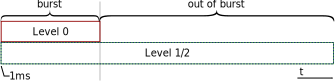
\includegraphics[width=0.9\textwidth]{bursttime-l12merged-eng}<2->
		\end{center}
	\end{figure}
\end{frame}



\subsection{New proposal}

\begin{frame}{Combine L1 and L2 to one farm}{}
	Data transmission via ordinary 10 gigabit ethernet and \textbf{UDP/IP}:
	\begin{center} 
		\includegraphics[width=0.8\textwidth]{merged-star-eng}
	\end{center} 
	\begin{exampleblock}{We save about 30\% hardware ($\gtrsim$100 k$\EUR$)}
		\begin{itemize}
		  \item No L1 PCs anymore
		  \item Less switches, less network cards
		\end{itemize}
	\end{exampleblock}
\end{frame}

\begin{frame}{New proposal}{Event building @ L1}
	\begin{center} 
		\includegraphics[width=0.6\textwidth]{dataflow-merged-gian-en}
	\end{center} 
	
	\begin{block}{Every subdetector sends data of one event to the same PC}
		\begin{itemize}
		  	\pro \textbf{More physics at earlier state}
		  	\pro No broadcast of a L1 decision needed anymore
		  	\pro Easier to implement load balancing (self-sustaining PCs)
%  			\contra Every farm PC must serve every subdetector $\Rightarrow$ needs
  			% GPUs
		\end{itemize}
	\end{block}
\end{frame}